\PassOptionsToPackage{unicode=true}{hyperref} % options for packages loaded elsewhere
\PassOptionsToPackage{hyphens}{url}
%
\documentclass[]{article}
\usepackage{lmodern}
\usepackage{amssymb,amsmath}
\usepackage{ifxetex,ifluatex}
\usepackage{fixltx2e} % provides \textsubscript
\ifnum 0\ifxetex 1\fi\ifluatex 1\fi=0 % if pdftex
  \usepackage[T1]{fontenc}
  \usepackage[utf8]{inputenc}
  \usepackage{textcomp} % provides euro and other symbols
\else % if luatex or xelatex
  \usepackage{unicode-math}
  \defaultfontfeatures{Ligatures=TeX,Scale=MatchLowercase}
\fi
% use upquote if available, for straight quotes in verbatim environments
\IfFileExists{upquote.sty}{\usepackage{upquote}}{}
% use microtype if available
\IfFileExists{microtype.sty}{%
\usepackage[]{microtype}
\UseMicrotypeSet[protrusion]{basicmath} % disable protrusion for tt fonts
}{}
\IfFileExists{parskip.sty}{%
\usepackage{parskip}
}{% else
\setlength{\parindent}{0pt}
\setlength{\parskip}{6pt plus 2pt minus 1pt}
}
\usepackage{hyperref}
\hypersetup{
            pdftitle={arc42 Template},
            pdfborder={0 0 0},
            breaklinks=true}
\urlstyle{same}  % don't use monospace font for urls
\usepackage{longtable,booktabs}
% Fix footnotes in tables (requires footnote package)
\IfFileExists{footnote.sty}{\usepackage{footnote}\makesavenoteenv{longtable}}{}
\usepackage{graphicx,grffile}
\makeatletter
\def\maxwidth{\ifdim\Gin@nat@width>\linewidth\linewidth\else\Gin@nat@width\fi}
\def\maxheight{\ifdim\Gin@nat@height>\textheight\textheight\else\Gin@nat@height\fi}
\makeatother
% Scale images if necessary, so that they will not overflow the page
% margins by default, and it is still possible to overwrite the defaults
% using explicit options in \includegraphics[width, height, ...]{}
\setkeys{Gin}{width=\maxwidth,height=\maxheight,keepaspectratio}
\setlength{\emergencystretch}{3em}  % prevent overfull lines
\providecommand{\tightlist}{%
  \setlength{\itemsep}{0pt}\setlength{\parskip}{0pt}}
\setcounter{secnumdepth}{0}
% Redefines (sub)paragraphs to behave more like sections
\ifx\paragraph\undefined\else
\let\oldparagraph\paragraph
\renewcommand{\paragraph}[1]{\oldparagraph{#1}\mbox{}}
\fi
\ifx\subparagraph\undefined\else
\let\oldsubparagraph\subparagraph
\renewcommand{\subparagraph}[1]{\oldsubparagraph{#1}\mbox{}}
\fi

% set default figure placement to htbp
\makeatletter
\def\fps@figure{htbp}
\makeatother


\title{
\includegraphics{images/arc42-logo.png} Template}
\date{2018-12-20}

\begin{document}
\maketitle

\section{}

\textbf{About arc42}

arc42, the Template for documentation of software and system
architecture.

By Dr. Gernot Starke, Dr. Peter Hruschka and contributors.

Template Revision: 7.0 EN (based on asciidoc), January 2017

© We acknowledge that this document uses material from the arc 42
architecture template, \url{http://www.arc42.de}. Created by Dr. Peter
Hruschka \& Dr. Gernot Starke.

\begin{quote}
\textbf{Note}

This version of the template contains some help and explanations. It is
used for familiarization with arc42 and the understanding of the
concepts. For documentation of your own system you use better the
\emph{plain} version.
\end{quote}

\hypertarget{section-introduction-and-goals}{%
\section{Introduction and Goals}\label{section-introduction-and-goals}}

Describes the relevant requirements and the driving forces that software
architects and development team must consider. These include

\begin{itemize}
\item
  underlying business goals, essential features and functional
  requirements for the system
\item
  quality goals for the architecture
\item
  relevant stakeholders and their expectations
\end{itemize}

\hypertarget{_requirements_overview}{%
\subsection{Requirements Overview}\label{_requirements_overview}}

\textbf{Contents.}

Short description of the functional requirements, driving forces,
extract (or abstract) of requirements. Link to (hopefully existing)
requirements documents (with version number and information where to
find it).

\textbf{Motivation.}

From the point of view of the end users a system is created or modified
to improve support of a business activity and/or improve the quality.

\textbf{Form.}

Short textual description, probably in tabular use-case format. If
requirements documents exist this overview should refer to these
documents.

Keep these excerpts as short as possible. Balance readability of this
document with potential redundancy w.r.t to requirements documents.

\hypertarget{_quality_goals}{%
\subsection{Quality Goals}\label{_quality_goals}}

\textbf{Contents.}

The top three (max five) quality goals for the architecture whose
fulfillment is of highest importance to the major stakeholders. We
really mean quality goals for the architecture. Don't confuse them with
project goals. They are not necessarily identical.

\textbf{Motivation.}

You should know the quality goals of your most important stakeholders,
since they will influence fundamental architectural decisions. Make sure
to be very concrete about these qualities, avoid buzzwords. If you as an
architect do not know how the quality of your work will be judged
\ldots{}

\textbf{Form.}

A table with quality goals and concrete scenarios, ordered by priorities

\hypertarget{_stakeholders}{%
\subsection{Stakeholders}\label{_stakeholders}}

\textbf{Contents.}

Explicit overview of stakeholders of the system, i.e. all person, roles
or organizations that

\begin{itemize}
\item
  should know the architecture
\item
  have to be convinced of the architecture
\item
  have to work with the architecture or with code
\item
  need the documentation of the architecture for their work
\item
  have to come up with decisions about the system or its development
\end{itemize}

\textbf{Motivation.}

You should know all parties involved in development of the system or
affected by the system. Otherwise, you may get nasty surprises later in
the development process. These stakeholders determine the extent and the
level of detail of your work and its results.

\textbf{Form.}

Table with role names, person names, and their expectations with respect
to the architecture and its documentation.

\begin{longtable}[]{@{}lll@{}}
\toprule
\begin{minipage}[b]{0.18\columnwidth}\raggedright
Role/Name\strut
\end{minipage} & \begin{minipage}[b]{0.37\columnwidth}\raggedright
Contact\strut
\end{minipage} & \begin{minipage}[b]{0.37\columnwidth}\raggedright
Expectations\strut
\end{minipage}\tabularnewline
\midrule
\endhead
\begin{minipage}[t]{0.18\columnwidth}\raggedright
\emph{\textless{}Role-1\textgreater{}}\strut
\end{minipage} & \begin{minipage}[t]{0.37\columnwidth}\raggedright
\emph{\textless{}Contact-1\textgreater{}}\strut
\end{minipage} & \begin{minipage}[t]{0.37\columnwidth}\raggedright
\emph{\textless{}Expectation-1\textgreater{}}\strut
\end{minipage}\tabularnewline
\begin{minipage}[t]{0.18\columnwidth}\raggedright
\emph{\textless{}Role-2\textgreater{}}\strut
\end{minipage} & \begin{minipage}[t]{0.37\columnwidth}\raggedright
\emph{\textless{}Contact-2\textgreater{}}\strut
\end{minipage} & \begin{minipage}[t]{0.37\columnwidth}\raggedright
\emph{\textless{}Expectation-2\textgreater{}}\strut
\end{minipage}\tabularnewline
\bottomrule
\end{longtable}

\hypertarget{section-architecture-constraints}{%
\section{Architecture
Constraints}\label{section-architecture-constraints}}

\textbf{Contents.}

Any requirement that constrains software architects in their freedom of
design and implementation decisions or decision about the development
process. These constraints sometimes go beyond individual systems and
are valid for whole organizations and companies.

\textbf{Motivation.}

Architects should know exactly where they are free in their design
decisions and where they must adhere to constraints. Constraints must
always be dealt with; they may be negotiable, though.

\textbf{Form.}

Simple tables of constraints with explanations. If needed you can
subdivide them into technical constraints, organizational and political
constraints and conventions (e.g. programming or versioning guidelines,
documentation or naming conventions)

\hypertarget{section-system-scope-and-context}{%
\section{System Scope and
Context}\label{section-system-scope-and-context}}

\textbf{Contents.}

System scope and context - as the name suggests - delimits your system
(i.e. your scope) from all its communication partners (neighboring
systems and users, i.e. the context of your system). It thereby
specifies the external interfaces.

If necessary, differentiate the business context (domain specific inputs
and outputs) from the technical context (channels, protocols, hardware).

\textbf{Motivation.}

The domain interfaces and technical interfaces to communication partners
are among your system's most critical aspects. Make sure that you
completely understand them.

\textbf{Form.}

Various options:

\begin{itemize}
\item
  Context diagrams
\item
  Lists of communication partners and their interfaces.
\end{itemize}

\hypertarget{_business_context}{%
\subsection{Business Context}\label{_business_context}}

\textbf{Contents.}

Specification of \textbf{all} communication partners (users, IT-systems,
\ldots{}) with explanations of domain specific inputs and outputs or
interfaces. Optionally you can add domain specific formats or
communication protocols.

\textbf{Motivation.}

All stakeholders should understand which data are exchanged with the
environment of the system.

\textbf{Form.}

All kinds of diagrams that show the system as a black box and specify
the domain interfaces to communication partners.

Alternatively (or additionally) you can use a table. The title of the
table is the name of your system, the three columns contain the name of
the communication partner, the inputs, and the outputs.

\textbf{\textless{}Diagram or Table\textgreater{}}

\textbf{\textless{}optionally: Explanation of external domain
interfaces\textgreater{}}

\hypertarget{_technical_context}{%
\subsection{Technical Context}\label{_technical_context}}

\textbf{Contents.}

Technical interfaces (channels and transmission media) linking your
system to its environment. In addition a mapping of domain specific
input/output to the channels, i.e. an explanation with I/O uses which
channel.

\textbf{Motivation.}

Many stakeholders make architectural decision based on the technical
interfaces between the system and its context. Especially infrastructure
or hardware designers decide these technical interfaces.

\textbf{Form.}

E.g. UML deployment diagram describing channels to neighboring systems,
together with a mapping table showing the relationships between channels
and input/output.

\textbf{\textless{}Diagram or Table\textgreater{}}

\textbf{\textless{}optionally: Explanation of technical
interfaces\textgreater{}}

\textbf{\textless{}Mapping Input/Output to Channels\textgreater{}}

\hypertarget{section-solution-strategy}{%
\section{Solution Strategy}\label{section-solution-strategy}}

\textbf{Contents.}

A short summary and explanation of the fundamental decisions and
solution strategies, that shape the system's architecture. These include

\begin{itemize}
\item
  technology decisions
\item
  decisions about the top-level decomposition of the system, e.g. 
  of an architectural pattern or design pattern
\item
  decisions on how to achieve key quality goals
\item
  relevant organizational decisions, e.g. selecting a development
  process or delegating certain tasks to third parties.
\end{itemize}

\textbf{Motivation.}

These decisions form the cornerstones for your architecture. They are
the basis for many other detailed decisions or implementation rules.

\textbf{Form.}

Keep the explanation of these key decisions short.

Motivate what you have decided and why you decided that way, based upon
your problem statement, the quality goals and key constraints. Refer to
details in the following sections.

\hypertarget{section-building-block-view}{%
\section{Building Block View}\label{section-building-block-view}}

\textbf{Content.}

The building block view shows the static decomposition of the system
into building blocks (modules, components, subsystems, classes,
interfaces, packages, libraries, frameworks, layers, partitions, tiers,
functions, macros, operations, datas structures, \ldots{}) as well as
their dependencies (relationships, associations, \ldots{})

This view is mandatory for every architecture documentation. In analogy
to a house this is the \emph{floor plan}.

\textbf{Motivation.}

Maintain an overview of your source code by making its structure
understandable through abstraction.

This allows you to communicate with your stakeholder on an abstract
level without disclosing implementation details.

\textbf{Form.}

The building block view is a hierarchical collection of black boxes and
white boxes (see figure below) and their descriptions.

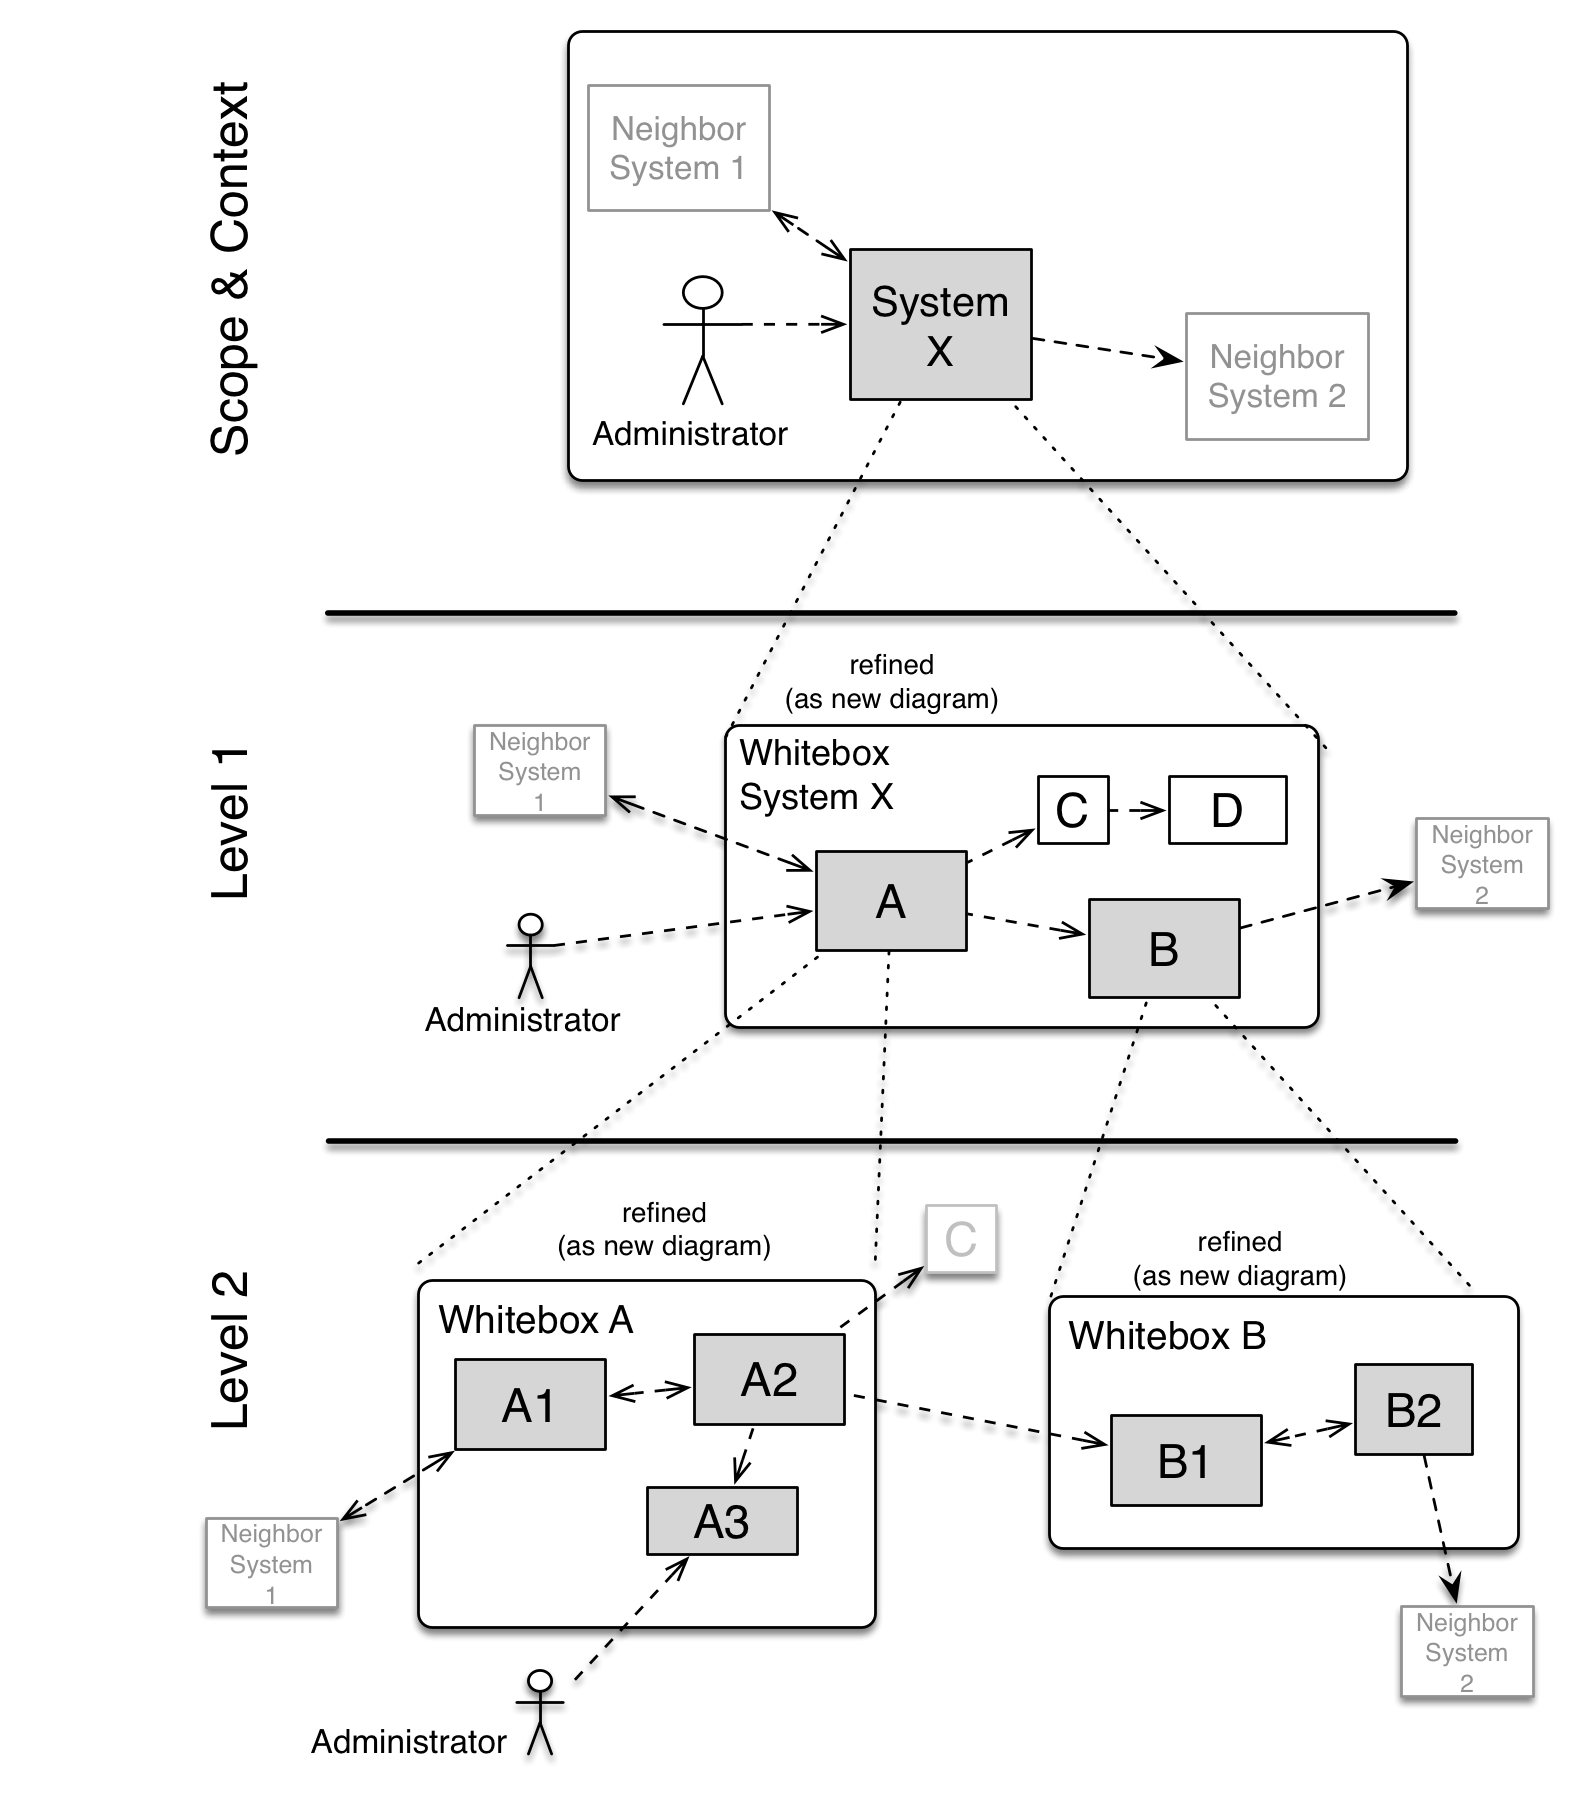
\includegraphics{images/05_building_blocks-EN.png}

\textbf{Level 1} is the white box description of the overall system
together with black box descriptions of all contained building blocks.

\textbf{Level 2} zooms into some building blocks of level 1. Thus it
contains the white box description of selected building blocks of level
1, together with black box descriptions of their internal building
blocks.

\textbf{Level 3} zooms into selected building blocks of level 2, and so
on.

\hypertarget{_whitebox_overall_system}{%
\subsection{Whitebox Overall System}\label{_whitebox_overall_system}}

Here you describe the decomposition of the overall system using the
following white box template. It contains

\begin{itemize}
\item
  an overview diagram
\item
  a motivation for the decomposition
\item
  black box descriptions of the contained building blocks. For these we
  offer you alternatives:

  \begin{itemize}
  \item
    use \emph{one} table for a short and pragmatic overview of all
    contained building blocks and their interfaces
  \item
    use a list of black box descriptions of the building blocks
    according to the black box template (see below). Depending on your
    choice of tool this list could be sub-chapters (in text files),
    sub-pages (in a Wiki) or nested elements (in a modeling tool).
  \end{itemize}
\item
  (optional:) important interfaces, that are not explained in the black
  box templates of a building block, but are very important for
  understanding the white box. Since there are so many ways to specify
  interfaces why do not provide a specific template for them. In the
  worst case you have to specify and describe syntax, semantics,
  protocols, error handling, restrictions, versions, qualities,
  necessary compatibilities and many things more. In the best case you
  will get away with examples or simple signatures.
\end{itemize}

\emph{\textbf{\textless{}Overview Diagram\textgreater{}}}

\begin{description}
\item[Motivation]
\emph{\textless{}text explanation\textgreater{}}
\item[Contained Building Blocks]
\emph{\textless{}Description of contained building block (black
boxes)\textgreater{}}
\item[Important Interfaces]
\emph{\textless{}Description of important interfaces\textgreater{}}
\end{description}

Insert your explanations of black boxes from level 1:

If you use tabular form you will only describe your black boxes with
name and responsibility according to the following schema:

\begin{longtable}[]{@{}ll@{}}
\toprule
\begin{minipage}[b]{0.31\columnwidth}\raggedright
\textbf{Name}\strut
\end{minipage} & \begin{minipage}[b]{0.63\columnwidth}\raggedright
\textbf{Responsibility}\strut
\end{minipage}\tabularnewline
\midrule
\endhead
\begin{minipage}[t]{0.31\columnwidth}\raggedright
\emph{\textless{}black box 1\textgreater{}}\strut
\end{minipage} & \begin{minipage}[t]{0.63\columnwidth}\raggedright
~\emph{\textless{}Text\textgreater{}}\strut
\end{minipage}\tabularnewline
\begin{minipage}[t]{0.31\columnwidth}\raggedright
\emph{\textless{}black box 2\textgreater{}}\strut
\end{minipage} & \begin{minipage}[t]{0.63\columnwidth}\raggedright
~\emph{\textless{}Text\textgreater{}}\strut
\end{minipage}\tabularnewline
\bottomrule
\end{longtable}

If you use a list of black box descriptions then you fill in a separate
black box template for every important building block . Its headline is
the name of the black box.

\hypertarget{__name_black_box_1}{%
\subsubsection{\textless{}Name black box
1\textgreater{}}\label{__name_black_box_1}}

Here you describe \textless{}black box 1\textgreater{} according the the
following black box template:

\begin{itemize}
\item
  Purpose/Responsibility
\item
  Interface(s), when they are not extracted as separate paragraphs. This
  interfaces may include qualities and performance characteristics.
\item
  (Optional) Quality-/Performance characteristics of the black box,
  e.g.availability, run time behavior, \ldots{}.
\item
  (Optional) directory/file location
\item
  (Optional) Fulfilled requirements (if you need traceability to
  requirements).
\item
  (Optional) Open issues/problems/risks
\end{itemize}

\emph{\textless{}Purpose/Responsibility\textgreater{}}

\emph{\textless{}Interface(s)\textgreater{}}

\emph{\textless{}(Optional) Quality/Performance
Characteristics\textgreater{}}

\emph{\textless{}(Optional) Directory/File Location\textgreater{}}

\emph{\textless{}(Optional) Fulfilled Requirements\textgreater{}}

\emph{\textless{}(optional) Open Issues/Problems/Risks\textgreater{}}

\hypertarget{__name_black_box_2}{%
\subsubsection{\textless{}Name black box
2\textgreater{}}\label{__name_black_box_2}}

\emph{\textless{}black box template\textgreater{}}

\hypertarget{__name_black_box_n}{%
\subsubsection{\textless{}Name black box
n\textgreater{}}\label{__name_black_box_n}}

\emph{\textless{}black box template\textgreater{}}

\hypertarget{__name_interface_1}{%
\subsubsection{\textless{}Name interface
1\textgreater{}}\label{__name_interface_1}}

\ldots{}

\hypertarget{__name_interface_m}{%
\subsubsection{\textless{}Name interface
m\textgreater{}}\label{__name_interface_m}}

\hypertarget{_level_2}{%
\subsection{Level 2}\label{_level_2}}

Here you can specify the inner structure of (some) building blocks from
level 1 as white boxes.

You have to decide which building blocks of your system are important
enough to justify such a detailed description. Please prefer relevance
over completeness. Specify important, surprising, risky, complex or
volatile building blocks. Leave out normal, simple, boring or
standardized parts of your system

\hypertarget{_white_box_emphasis_building_block_1_emphasis}{%
\subsubsection{\texorpdfstring{White Box \emph{\textless{}building block
1\textgreater{}}}{White Box \textless{}building block 1\textgreater{}}}\label{_white_box_emphasis_building_block_1_emphasis}}

\ldots{}describes the internal structure of \emph{building block 1}.

\emph{\textless{}white box template\textgreater{}}

\hypertarget{_white_box_emphasis_building_block_2_emphasis}{%
\subsubsection{\texorpdfstring{White Box \emph{\textless{}building block
2\textgreater{}}}{White Box \textless{}building block 2\textgreater{}}}\label{_white_box_emphasis_building_block_2_emphasis}}

\emph{\textless{}white box template\textgreater{}}

\ldots{}

\hypertarget{_white_box_emphasis_building_block_m_emphasis}{%
\subsubsection{\texorpdfstring{White Box \emph{\textless{}building block
m\textgreater{}}}{White Box \textless{}building block m\textgreater{}}}\label{_white_box_emphasis_building_block_m_emphasis}}

\emph{\textless{}white box template\textgreater{}}

\hypertarget{_level_3}{%
\subsection{Level 3}\label{_level_3}}

Here you can specify the inner structure of (some) building blocks from
level 2 as white boxes.

When you need more detailed levels of your architecture please copy this
part of arc42 for additional levels.

\hypertarget{_white_box_building_block_x_1}{%
\subsubsection{White Box \textless{}\_building block
x.1\_\textgreater{}}\label{_white_box_building_block_x_1}}

Specifies the internal structure of \emph{building block x.1}.

\emph{\textless{}white box template\textgreater{}}

\hypertarget{_white_box_building_block_x_2}{%
\subsubsection{White Box \textless{}\_building block
x.2\_\textgreater{}}\label{_white_box_building_block_x_2}}

\emph{\textless{}white box template\textgreater{}}

\hypertarget{_white_box_building_block_y_1}{%
\subsubsection{White Box \textless{}\_building block
y.1\_\textgreater{}}\label{_white_box_building_block_y_1}}

\emph{\textless{}white box template\textgreater{}}

\hypertarget{section-runtime-view}{%
\section{Runtime View}\label{section-runtime-view}}

\textbf{Contents.}

The runtime view describes concrete behavior and interactions of the
system's building blocks in form of scenarios from the following areas:

\begin{itemize}
\item
  important use cases or features: how do building blocks execute them?
\item
  interactions at critical external interfaces: how do building blocks
  cooperate with users and neighboring systems?
\item
  operation and administration: launch, start-up, stop
\item
  error and exception scenarios
\end{itemize}

Remark: The main criterion for the choice of possible scenarios
(sequences, workflows) is their \textbf{architectural relevance}. It is
\textbf{not} important to describe a large number of scenarios. You
should rather document a representative selection.

\textbf{Motivation.}

You should understand how (instances of) building blocks of your system
perform their job and communicate at runtime. You will mainly capture
scenarios in your documentation to communicate your architecture to
stakeholders that are less willing or able to read and understand the
static models (building block view, deployment view).

\textbf{Form.}

There are many notations for describing scenarios, e.g.

\begin{itemize}
\item
  numbered list of steps (in natural language)
\item
  activity diagrams or flow charts
\item
  sequence diagrams
\item
  BPMN or EPCs (event process chains)
\item
  state machines
\item
  \ldots{}
\end{itemize}

\hypertarget{__runtime_scenario_1}{%
\subsection{\textless{}Runtime Scenario
1\textgreater{}}\label{__runtime_scenario_1}}

\begin{itemize}
\item
  \emph{\textless{}insert runtime diagram or textual description of the
  scenario\textgreater{}}
\item
  \emph{\textless{}insert description of the notable aspects of the
  interactions between the building block instances depicted in this
  diagram.\textgreater{}}
\end{itemize}

\hypertarget{__runtime_scenario_2}{%
\subsection{\textless{}Runtime Scenario
2\textgreater{}}\label{__runtime_scenario_2}}

\hypertarget{_}{%
\subsection{\ldots{}}\label{_}}

\hypertarget{__runtime_scenario_n}{%
\subsection{\textless{}Runtime Scenario
n\textgreater{}}\label{__runtime_scenario_n}}

\hypertarget{section-deployment-view}{%
\section{Deployment View}\label{section-deployment-view}}

\textbf{Content.}

The deployment view describes:

\begin{enumerate}
\def\labelenumi{\arabic{enumi}.}
\item
  the technical infrastructure used to execute your system, with
  infrastructure elements like geographical locations, environments,
  computers, processors, channels and net topologies as well as other
  infrastructure elements and
\item
  the mapping of (software) building blocks to that infrastructure
  elements.
\end{enumerate}

Often systems are executed in different environments, e.g. development
environment, test environment, production environment. In such cases you
should document all relevant environments.

Especially document the deployment view when your software is executed
as distributed system with more then one computer, processor, server or
container or when you design and construct your own hardware processors
and chips.

From a software perspective it is sufficient to capture those elements
of the infrastructure that are needed to show the deployment of your
building blocks. Hardware architects can go beyond that and describe the
infrastructure to any level of detail they need to capture.

\textbf{Motivation.}

Software does not run without hardware. This underlying infrastructure
can and will influence your system and/or some cross-cutting concepts.
Therefore, you need to know the infrastructure.

Maybe the highest level deployment diagram is already contained in
section 3.2. as technical context with your own infrastructure as ONE
black box. In this section you will zoom into this black box using
additional deployment diagrams:

\begin{itemize}
\item
  UML offers deployment diagrams to express that view. Use it, probably
  with nested diagrams, when your infrastructure is more complex.
\item
  When your (hardware) stakeholders prefer other kinds of diagrams
  rather than the deployment diagram, let them use any kind that is able
  to show nodes and channels of the infrastructure.
\end{itemize}

\hypertarget{_infrastructure_level_1}{%
\subsection{Infrastructure Level 1}\label{_infrastructure_level_1}}

Describe (usually in a combination of diagrams, tables, and text):

\begin{itemize}
\item
  the distribution of your system to multiple locations, environments,
  computers, processors, .. as well as the physical connections between
  them
\item
  important justification or motivation for this deployment structure
\item
  Quality and/or performance features of the infrastructure
\item
  the mapping of software artifacts to elements of the infrastructure
\end{itemize}

For multiple environments or alternative deployments please copy that
section of arc42 for all relevant environments.

\emph{\textbf{\textless{}Overview Diagram\textgreater{}}}

\begin{description}
\item[Motivation]
\emph{\textless{}explanation in text form\textgreater{}}
\item[Quality and/or Performance Features]
\emph{\textless{}explanation in text form\textgreater{}}
\item[Mapping of Building Blocks to Infrastructure]
\emph{\textless{}description of the mapping\textgreater{}}
\end{description}

\hypertarget{_infrastructure_level_2}{%
\subsection{Infrastructure Level 2}\label{_infrastructure_level_2}}

Here you can include the internal structure of (some) infrastructure
elements from level 1.

Please copy the structure from level 1 for each selected element.

\hypertarget{__emphasis_infrastructure_element_1_emphasis}{%
\subsubsection{\texorpdfstring{\emph{\textless{}Infrastructure Element
1\textgreater{}}}{\textless{}Infrastructure Element 1\textgreater{}}}\label{__emphasis_infrastructure_element_1_emphasis}}

\emph{\textless{}diagram + explanation\textgreater{}}

\hypertarget{__emphasis_infrastructure_element_2_emphasis}{%
\subsubsection{\texorpdfstring{\emph{\textless{}Infrastructure Element
2\textgreater{}}}{\textless{}Infrastructure Element 2\textgreater{}}}\label{__emphasis_infrastructure_element_2_emphasis}}

\emph{\textless{}diagram + explanation\textgreater{}}

\ldots{}

\hypertarget{__emphasis_infrastructure_element_n_emphasis}{%
\subsubsection{\texorpdfstring{\emph{\textless{}Infrastructure Element
n\textgreater{}}}{\textless{}Infrastructure Element n\textgreater{}}}\label{__emphasis_infrastructure_element_n_emphasis}}

\emph{\textless{}diagram + explanation\textgreater{}}

\hypertarget{section-concepts}{%
\section{Cross-cutting Concepts}\label{section-concepts}}

\textbf{Content.}

This section describes overall, principal regulations and solution ideas
that are relevant in multiple parts (= cross-cutting) of your system.
Such concepts are often related to multiple building blocks. They can
include many different topics, such as

\begin{itemize}
\item
  domain models
\item
  architecture patterns or design patterns
\item
  rules for using specific technology
\item
  principal, often technical decisions of overall decisions
\item
  implementation rules
\end{itemize}

\textbf{Motivation.}

Concepts form the basis for \emph{conceptual integrity} (consistency,
homogeneity) of the architecture. Thus, they are an important
contribution to achieve inner qualities of your system.

Some of these concepts cannot be assigned to individual building blocks
(e.g. security or safety). This is the place in the template that we
provided for a cohesive specification of such concepts.

\textbf{Form.}

The form can be varied:

\begin{itemize}
\item
  concept papers with any kind of structure
\item
  cross-cutting model excerpts or scenarios using notations of the
  architecture views
\item
  sample implementations, especially for technical concepts
\item
  reference to typical usage of standard frameworks (e.g. using
  Hibernate for object/relational mapping)
\end{itemize}

\textbf{Structure.}

A potential (but not mandatory) structure for this section could be:

\begin{itemize}
\item
  Domain concepts
\item
  User Experience concepts (UX)
\item
  Safety and security concepts
\item
  Architecture and design patterns
\item
  "Under-the-hood"
\item
  development concepts
\item
  operational concepts
\end{itemize}

Note: it might be difficult to assign individual concepts to one
specific topic on this list.

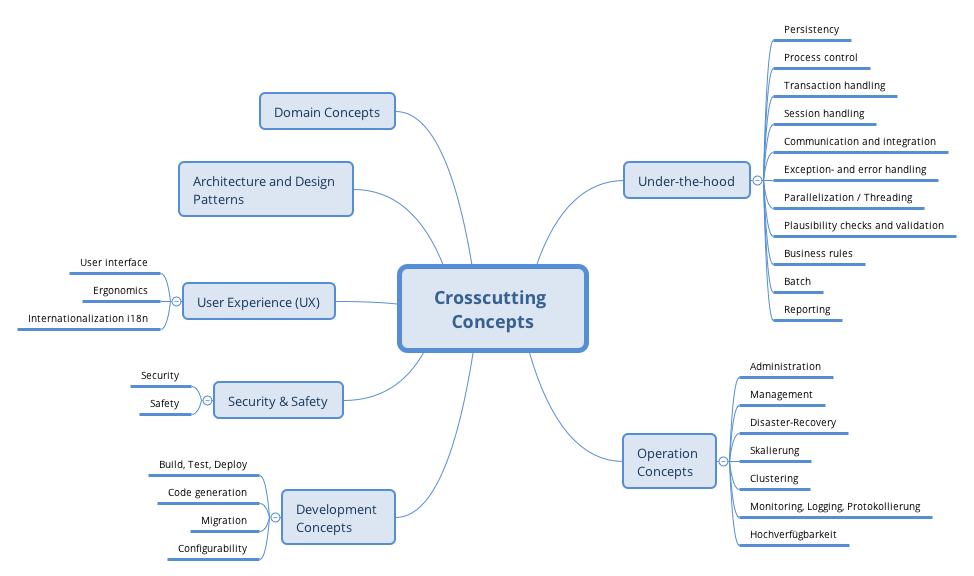
\includegraphics{images/08-Crosscutting-Concepts-Structure-EN.png}

\hypertarget{__emphasis_concept_1_emphasis}{%
\subsection{\texorpdfstring{\emph{\textless{}Concept
1\textgreater{}}}{\textless{}Concept 1\textgreater{}}}\label{__emphasis_concept_1_emphasis}}

\emph{\textless{}explanation\textgreater{}}

\hypertarget{__emphasis_concept_2_emphasis}{%
\subsection{\texorpdfstring{\emph{\textless{}Concept
2\textgreater{}}}{\textless{}Concept 2\textgreater{}}}\label{__emphasis_concept_2_emphasis}}

\emph{\textless{}explanation\textgreater{}}

\ldots{}

\hypertarget{__emphasis_concept_n_emphasis}{%
\subsection{\texorpdfstring{\emph{\textless{}Concept
n\textgreater{}}}{\textless{}Concept n\textgreater{}}}\label{__emphasis_concept_n_emphasis}}

\emph{\textless{}explanation\textgreater{}}

\hypertarget{section-design-decisions}{%
\section{Design Decisions}\label{section-design-decisions}}

\textbf{Contents.}

Important, expensive, large scale or risky architecture decisions
including rationals. With "decisions" we mean selecting one alternative
based on given criteria.

Please use your judgement to decide whether an architectural decision
should be documented here in this central section or whether you better
document it locally (e.g. within the white box template of one building
block).

Avoid redundancy. Refer to section 4, where you already captured the
most important decisions of your architecture.

\textbf{Motivation.}

Stakeholders of your system should be able to comprehend and retrace
your decisions.

\textbf{Form.}

Various options:

\begin{itemize}
\item
  List or table, ordered by importance and consequences or:
\item
  more detailed in form of separate sections per decision
\item
  ADR (architecture decision record) for every important decision
\end{itemize}

\hypertarget{section-quality-scenarios}{%
\section{Quality Requirements}\label{section-quality-scenarios}}

\textbf{Content.}

This section contains all quality requirements as quality tree with
scenarios. The most important ones have already been described in
section 1.2. (quality goals)

Here you can also capture quality requirements with lesser priority,
which will not create high risks when they are not fully achieved.

\textbf{Motivation.}

Since quality requirements will have a lot of influence on architectural
decisions you should know for every stakeholder what is really important
to them, concrete and measurable.

\hypertarget{_quality_tree}{%
\subsection{Quality Tree}\label{_quality_tree}}

\textbf{Content.}

The quality tree (as defined in ATAM -- Architecture Tradeoff Analysis
Method) with quality/evaluation scenarios as leafs.

\textbf{Motivation.}

The tree structure with priorities provides an overview for a sometimes
large number of quality requirements.

\textbf{Form.}

The quality tree is a high-level overview of the quality goals and
requirements:

\begin{itemize}
\item
  tree-like refinement of the term "quality". Use "quality" or
  "usefulness" as a root
\item
  a mind map with quality categories as main branches
\end{itemize}

In any case the tree should include links to the scenarios of the
following section.

\hypertarget{_quality_scenarios}{%
\subsection{Quality Scenarios}\label{_quality_scenarios}}

\textbf{Contents.}

Concretization of (sometimes vague or implicit) quality requirements
using (quality) scenarios.

These scenarios describe what should happen when a stimulus arrives at
the system.

For architects, two kinds of scenarios are important:

\begin{itemize}
\item
  Usage scenarios (also called application scenarios or use case
  scenarios) describe the system's runtime reaction to a certain
  stimulus. This also includes scenarios that describe the system's
  efficiency or performance. Example: The system reacts to a user's
  request within one second.
\item
  Change scenarios describe a modification of the system or of its
  immediate environment. Example: Additional functionality is
  implemented or requirements for a quality attribute change.
\end{itemize}

\textbf{Motivation.}

Scenarios make quality requirements concrete and allow to more easily
measure or decide whether they are fulfilled.

Especially when you want to assess your architecture using methods like
ATAM you need to describe your quality goals (from section 1.2) more
precisely down to a level of scenarios that can be discussed and
evaluated.

\textbf{Form.}

Tabular or free form text.

\hypertarget{section-technical-risks}{%
\section{Risks and Technical Debts}\label{section-technical-risks}}

\textbf{Contents.}

A list of identified technical risks or technical debts, ordered by
priority

\textbf{Motivation.}

``Risk management is project management for grown-ups'' (Tim Lister,
Atlantic Systems Guild.)

This should be your motto for systematic detection and evaluation of
risks and technical debts in the architecture, which will be needed by
management stakeholders (e.g. project managers, product owners) as part
of the overall risk analysis and measurement planning.

\textbf{Form.}

List of risks and/or technical debts, probably including suggested
measures to minimize, mitigate or avoid risks or reduce technical debts.

\hypertarget{section-glossary}{%
\section{Glossary}\label{section-glossary}}

\textbf{Contents.}

The most important domain and technical terms that your stakeholders use
when discussing the system.

You can also see the glossary as source for translations if you work in
multi-language teams.

\textbf{Motivation.}

You should clearly define your terms, so that all stakeholders

\begin{itemize}
\item
  have an identical understanding of these terms
\item
  do not use synonyms and homonyms
\end{itemize}

\textbf{Form.}

A table with columns \textless{}Term\textgreater{} and
\textless{}Definition\textgreater{}.

Potentially more columns in case you need translations.

\begin{longtable}[]{@{}ll@{}}
\toprule
\begin{minipage}[b]{0.47\columnwidth}\raggedright
Term\strut
\end{minipage} & \begin{minipage}[b]{0.47\columnwidth}\raggedright
Definition\strut
\end{minipage}\tabularnewline
\midrule
\endhead
\begin{minipage}[t]{0.47\columnwidth}\raggedright
\textless{}Term-1\textgreater{}\strut
\end{minipage} & \begin{minipage}[t]{0.47\columnwidth}\raggedright
\textless{}definition-1\textgreater{}\strut
\end{minipage}\tabularnewline
\begin{minipage}[t]{0.47\columnwidth}\raggedright
\textless{}Term-2\textgreater{}\strut
\end{minipage} & \begin{minipage}[t]{0.47\columnwidth}\raggedright
\textless{}definition-2\textgreater{}\strut
\end{minipage}\tabularnewline
\bottomrule
\end{longtable}

\end{document}
